\documentclass{standalone}
\usepackage{tikz} % Import the tikz package
\usetikzlibrary{automata} % Import library for drawing automata
\usetikzlibrary{positioning} % ...positioning nodes
\usetikzlibrary{arrows} % ...customizing arrows
\tikzset{node distance=2.5cm,
    every state/.style={
        semithick,
        fill=gray!10},
    initial text={},
    double distance=2pt,
    every edge/.style={
        draw,
        ->,>=stealth',
        auto,
        semithick}}
\let\epsilon\varepsilon
\begin{document}
    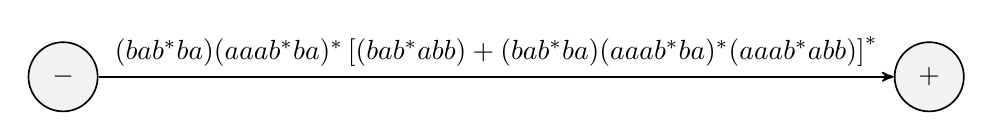
\begin{tikzpicture}
        \node[state] (start) at (0,0) {$-$};
        %\node[state,] (ul) at (2,0) {$1$};
        \node[state] (end) at (11,0) {$+$};

        \draw (start) edge[] node {$(bab^*ba)(aaab^*ba)^*\left[(bab^*abb)+(bab^*ba)(aaab^*ba)^*(aaab^*abb)\right]^*$} (end); 
        %\draw (ul) edge[] node {$(bab^*ba)(aaab^*bba)^*$} (end);
        %\draw (ul) edge[loop below] node {$(bab^*abb)+(bab^*ba)(aaab^*ba)^*(aaab^*abb)$} (ul);
    \end{tikzpicture}
\end{document}